\section{接口物理学：介质的流变学谱系与速率失配}

上一章讨论的可达空间，解决的是哪些状态能够被系统稳定抵达。但路径只描述通道，不描述穿过通道时智能输入会变成什么。同一条被打开的路径，在不同介质中会得到不同的响应：有的迅速扩散，有的必须做功，有的会反弹回来。介质不是路径的附属条件，它决定输入能否变成状态改变。

智能不是直接改变世界，而是被介质转译。这是理解 AI 进入现实系统时最容易被忽略的一点。人们习惯说“AI 会改变世界”，但世界并不是一种均匀材料。文本、代码、图像、机器、道路、药物、细胞、身体和生态系统，并不会以同一种方式接收智能输入。同样一个模型输出，在文本系统中可以迅速扩散，在机器人系统中必须变成力和运动，在生命系统中则会触发代谢、免疫、代偿、适应甚至反弹。因此，AI 的真实效能，不只取决于模型本身有多强，还取决于它的输出被何种介质吸收；智能输入只有经过介质转译，才会成为现实改变，转译稳定，智能就变成有效功，转译失配，智能就变成噪声、热、磨损、震荡、验证负担或系统反抗。这就是\term{介质响应谱}：不同介质面对智能输入时，将其转化为状态变化的方式。比特把智能转译为扩散，原子把智能转译为做功，生命把智能转译为反馈。三者不是三类普通应用场景，而是三种不同的吸收机制：比特关心复制、组合和传播，原子关心能量、惯性和耗散，生命关心代谢、调节和适应。用同一种智能加速逻辑驱动三种介质，必然产生错觉。

\subsection{三条响应谱：比特扩散、原子做功、生命反馈}

\subhead{比特介质的扩散响应}

比特介质的基本响应是扩散。在比特域中，智能输入最容易转化为新的信息结构：一段文字、一张图像、一组代码、一个模型输出、一个设计草案、一个搜索结果。它们可以被快速复制、修改、分发、组合和再生成。比特介质的特殊性在于，状态改变主要表现为符号排列改变，而不是物质位置改变。正因如此，AI 在比特域中最容易爆发，它可以用极低边际成本生成大量内容，把过去需要人类长时间表达、检索、改写和组合的任务迅速压缩。

但是，扩散不是证明。比特介质的低黏滞主要发生在横向传播层面，而不是纵向确证层面。横向传播是复制更多、生成更多、分发更快、组合更密；纵向确证则要求信息更真实、更可靠、更有来源、更可解释、更能承受责任。前者很容易被 AI 放大，后者却不会因为生成速度提高而自动变轻。文本可以快速生成，但事实仍要核查；图像可以快速生成，但来源仍要追踪；代码可以快速生成，但安全和维护仍要审计；观点可以快速扩散，但公共信任不会自动增长。

所以，比特介质的核心矛盾不是能不能生成，而是能不能变真。它可以低成本扩展可能性，却不能低成本保证真实性。生成越便宜，可信结果越稀缺；内容越多，筛选越重；表达越顺滑，判断越重要。比特把智能转译为扩散，但扩散之后会制造新的确证压力，而压力并不落在生成端，它落在确证端。

比特还依赖现实作为锚点。模型的智能并不是在纯逻辑闭环中凭空生长，而是来自对现实世界的压缩：真实语言、真实图像、真实实验、真实代码、真实行为、真实反馈。比特世界看起来轻，是因为它把现实转化成了可复制的信息结构，但这种可复制性不能脱离现实来源。若信息系统越来越多地吞噬自身生成的内容，而缺少新的现实摩擦和外部反馈，它会变得越来越顺滑，也可能越来越封闭\cite{shumailov2024ai}。它可以产生一致性，却未必产生真实性；可以提高流畅度，却可能降低方差和外部校准。

因此，比特介质不是无黏滞介质，而是将黏滞隐藏在两个地方：一是物理后台，二是现实确证。前者包括芯片、电力、冷却、数据中心和网络基础设施；后者包括真实数据、事实核查、人工反馈、来源追踪和责任机制。用户看到的是低成本扩散，系统支付的是后台资源和验证成本。比特扩散得越快，越需要现实来校准它。而当输出要改变的已经不是符号排列，而是物质位置时，介质的响应方式随之更换。

\subhead{原子介质的做功响应}

原子介质的基本响应是做功。原子世界不会因为一个信息结构被生成就自动改变，控制信号必须变成能量流，路径规划必须变成运动，设计图必须变成材料、加工、装配、测试和维护。原子介质不关心一个方案在符号空间中多优雅，它只关心这个方案能否在力、热、摩擦、惯性、材料强度和空间约束中执行。原子把智能输入转译为物理作用，这个转译过程总要支付能量、承受耗散，并受制于时间。搬运需要力，制造需要工艺，冷却需要热交换，运动需要控制，建筑需要材料，机器人需要电机和关节，电网需要容量和稳定性。AI 可以优化路径，但不能取消质量；可以减少试错，但不能取消做功；可以提高调度效率，但不能取消容量限制；可以增强控制，但不能取消摩擦、磨损、热和失效。

因此，原子介质不是被智能“说服”的介质，而是被智能“驱动”的介质。比特扩散可以接近瞬时，原子响应必须经历能量转移和结构改变。一个更聪明的机器人策略，仍然需要执行器输出力矩；一个更优的物流调度，仍然需要车辆、道路、仓储和装卸；一个更精密的芯片设计，仍然需要洁净室、光刻、材料、缺陷控制和散热。智能在这里不是直接变成结果，而是变成对物理过程的控制。这也是为什么原子介质具有相对稳定的耗散残余：输入不可能全部变成有效功，总会有一部分变成热、磨损、噪声、误差和维护负担。控制越精密，传感和执行成本越高；速度越快，功率和热管理压力越大；系统越复杂，校准和维护越重。原子世界并不拒绝智能，但它要求智能遵守能量、功率、热、材料和失效的账本。

原子介质还有响应带宽。物理系统不能无限高频改变状态：机器有惯性，材料有疲劳，热有扩散时间，执行器有响应极限，电网有稳定约束，交通有刹车距离和反应延迟。AI 可以高频生成控制建议，但原子介质未必能够同频吸收。输入太快，不会自动变成更多有效功，反而可能变成震荡、过调节、发热、磨损和安全风险。

所以，原子介质中的智能价值，不在于把比特速度强加给物质，而在于找到合适的驱动方式。好的物理智能必须知道介质能承受什么功率、什么频率、什么误差、什么反馈延迟。它不是简单追求更快输出，而是让输出与物理响应匹配；不是每一刻都生成新方案，而是让控制进入稳定闭环；不是追求符号最优，而是追求可执行、低耗散、可维护和可恢复。原子把智能转译为做功，也把智能暴露在物理损耗中，一个不能管理热、磨损、误差和维护的智能系统，模型再强，也只能停留在演示阶段。原子介质要求智能从“答案”下降为“动作”，从“方案”下降为“过程”，从“最优”下降为“可长期运行”。做功的对象不会回应输入。一旦介质自身开始解释输入，并据此调整内部状态，转译就进入第三层。

\subhead{生命介质的反馈响应}

生命介质的基本响应是反馈。生命当然也是物质，但它不是普通物质：普通原子系统主要承受外部作用，生命系统则会解释外部作用，它有边界，有代谢，有防御，有修复，有调节，有记忆，有适应。药物不是简单施加在靶点上，而是进入代谢网络、免疫系统、组织环境和行为背景；基因编辑不是改写一串字符，而是扰动发育过程、表达调控、细胞环境和生态关系；医疗干预不是单向控制身体，而是与身体自身的反馈系统共同作用。

所以，生命介质不是被动执行智能输入，而是把输入当成扰动。它会吸收一部分，抵消一部分，放大一部分，延迟一部分，反弹一部分。外部干预越强、越快、越粗暴，生命系统未必越快被改变，反而可能激发更强阻抗。免疫反应、炎症、耐药性、代偿机制、内分泌反调节、生态反弹，都说明生命系统不是线性负载，而是有自我维持倾向的复杂适应系统。流变学里有一类介质，在低速扰动下可以流动，在高速强扰动下反而变硬\cite{brown2014shear}。生命系统也有类似响应，低强度、低频率、可适应的干预，可能被系统柔性吸收，而高频、强力、跨尺度的干预，则可能让阻力突然上升。不是因为生命系统神秘，而是因为它内部有多层反馈，外部驱动超过系统自身弛豫时间，就会打破调节节奏，引发防御、代偿或失稳。

这解释了为什么生命不能像软件一样快速迭代。软件可以多版本试错，人体不能无限试错；代码错误可以回滚，生命干预不能轻易回滚；模型可以高频更新，生理反馈需要时间展开；短期指标可以被优化，长期副作用却可能延迟出现。生命介质的反馈不总是即时的，它常把后果藏在时间里：一个干预今天看似有效，可能几个月后被代偿机制抵消；一个指标短期改善，可能几年后暴露系统代价。生命介质的非线性也意味着，局部目标不能直接等同于系统目标。降低一个指标，不一定改善身体状态；激活一个通路，不一定带来全局收益；压制一种反应，可能释放另一种风险；编辑一个基因，可能牵动发育、表达和生态背景。生命系统中的“作用点”从来不是孤立点，而是网络中的节点，智能可以找到更精细的切入点，但不能让生命系统停止反馈。

因此，AI 在生命科学中的作用会高度不均匀。它可以快速扩大候选空间：发现靶点，预测结构，生成分子，设计实验，识别模式。但生命介质不会以同样速度承认这些候选：候选分子可以大量生成，药物不能大量上市；基因编辑方案可以迅速设计，安全性不能迅速证明；诊断模型可以快速训练，临床责任不能自动消失。AI 可以加速发现，却不能取消生命反馈。生命把智能转译为反馈，也把智能推入长期验证。原子系统的失败常表现为磨损、断裂、发热、失稳，生命系统的失败可能表现为代偿、耐受、迟发副作用、群体差异、行为改变和生态后果。它不只有物理损耗，还有适应性回应，原子主要承受力，生命会回应力。

响应可以先用三个典型模型描述：一阶跟随、带启动延迟的限速推进、欠阻尼反馈。设$y(t)$为选定结果的响应，$y_\infty$为对应的稳态值，三个模型分别写为
\begin{align}
y_{b}(t)&=y_{\infty}\bigl(1-e^{-t/\tau_{b}}\bigr),\qquad \tau_{b}\to 0^{+}\label{eq:resp-bit}\\[2pt]
y_{a}(t)&=y_{\infty}\min\left\{\frac{(t-t_{d})_{+}}{\tau_{a}},\;1\right\},\qquad t_{d}>0\label{eq:resp-atom}\\[2pt]
y_{l}(t)&=y_{\infty}\left[1-e^{-\zeta\omega t}\left(\cos\omega_{d}t+\frac{\zeta}{\sqrt{1-\zeta^{2}}}\sin\omega_{d}t\right)\right],\qquad 0<\zeta<1\label{eq:resp-life}
\end{align}
三式中的时间参数采用同一单位，响应以相同参照值归一化。第一式的$\tau_b$是一阶时间常数；第二式的$t_d$为启动延迟，$\tau_a$控制限速推进的时长；第三式的$\zeta$为阻尼比，$\omega$为自然角频率，$\omega_d=\omega\sqrt{1-\zeta^2}$。当$0<\zeta<1$时，第三式出现超调，并逐渐回到稳态。这些形式适合描述相应任务中的快速跟随、产能限制和反馈回落；参数和形式须按响应数据选择。

介质分析为选取模型提供机制线索。数字分发常有较短的响应时间，制造常受启动与通量限制，生物干预常伴随代偿和迟滞。同一介质也可以出现多种响应：信息网络会拥塞，机械系统会超调，生命过程可以单调趋近。比较的对象是具体通道的响应，而非由介质名称预先指定的曲线。
\begin{figure}[ht]
\centering
% >>>>>>>>>> figs/fig-three-media.tex >>>>>>>>>>
% 图 3-1  三种介质的响应谱：扩散、做功、反馈
% 横轴对数时间，纵轴归一化响应。三条曲线画在同一套坐标上，
% 因此差异一眼可见——它们不是三种应用场景，是三种吸收机制。
%
% 曲线来自 figs/_curve-three-media.tex（\input 必须带 figs/ 前缀，
% 因为本图会被 make_book.py 并进书稿根目录下的那个整文件里，
% 不带前缀的路径在那里的相对位置是不对的），由 _sim_three_media.py 算出来，
% 是 ch03 式 (3.1) 组的数值解。这一点很重要：本图原来的三条线是拿 8--11 个
% 控制点 smooth 出来的，其中「比特冲高后单调衰减」「生命过冲后跌破零线」
% 两条都与式 (3.1) 不符——一阶阶跃响应单调升到 y_inf 并停住；
% 二阶欠阻尼阶跃响应的极小值是 y_inf(1-exp(-pi*zeta/sqrt(1-zeta^2))^2)，
% 对 zeta=0.18 是 0.685，恒为正，不可能转负。图与式子必须说同一件事。
%
% 三条曲线最终都落在 y_inf 上，所以右侧有一大段三线重合——
% 这不是画漏了，正是式子要说的事：介质之间的差别全在到达的过程里。
\begin{tikzpicture}[x=1cm, y=1cm, font=\small,
  ax/.style={-{Stealth[length=2.0mm]}, ink, line width=0.6pt},
  tk/.style={font=\scriptsize, text=slate, anchor=north},
  yk/.style={font=\scriptsize, text=slate, anchor=east}
]
\useasboundingbox (-0.85,1.45) rectangle (11.20,-5.90);

\def\aX{1.00} \def\aY{-4.30} \def\dx{1.15} \def\dy{3.15} \def\aR{9.90}
% 横坐标以 log10(t) 记：\lgt{-2} 是 10^{-2} s
% 展开成 \dx*2+\dx*#1 而不是 \dx*(#1+2)：坐标里一旦出现紧跟乘号的左括号，
% pgf 会把它当成节点名去查，报「No shape named 1 is known」。
% 同理，坐标宏里不要出现「* ( 数字 )」这种写法。
\def\lgt#1{\aX+\dx*2+\dx*#1}
\def\py#1{\aY+\dy*#1}

\draw[ax] (\aX,\aY) -- (\aR,\aY)
      node[anchor=north east, font=\scriptsize, text=ink, yshift=-1pt] {时间 $t$ (s)};
\draw[ax] (\aX,\aY) -- (\aX,{\py{1.80}})
      node[anchor=south, font=\scriptsize, text=ink, yshift=1pt] {归一化响应};

% ---------- 刻度 ----------
\foreach \e/\t in {-2/{$10^{-2}$},0/{1},2/{$10^{2}$},4/{$10^{4}$}} {
  \draw[slate!55, line width=0.4pt] (\lgt{\e},\aY) -- (\lgt{\e},\aY-0.07);
  \node[tk] at (\lgt{\e},\aY-0.10) {\t};
}
\foreach \f in {0,0.5,1.0,1.5} {
  \draw[slate!55, line width=0.4pt] (\aX,\py{\f}) -- ({\aX-0.07},\py{\f});
  \node[yk] at ({\aX-0.09},\py{\f}) {\f};
}
% 稳态线：三条曲线最终都落在它上面
\draw[slate!70, line width=0.6pt] (\aX,\py{1.0}) -- (\aR,\py{1.0});
\node[font=\scriptsize, text=slate, anchor=south east] at (\lgt{0.95},\py{1.02})
      {稳态 $y_\infty$};

% ---------- 三条响应曲线（ch03 式 3.1 的数值解）----------
% >>>>>>>>>> figs/_curve-three-media.tex >>>>>>>>>>
% 本文件由 _sim_three_media.py 生成，不要手改。
% 三条曲线是 ch03 式 (3.1) 组的数值解，不是手画的形状。
% tau_b=5e-03 s, t_d=1 s, tau_a=100 s, zeta=0.18, 首个峰在 700 s

\draw[deepblue!85, line width=1.5pt] plot[smooth, tension=0.45]
  coordinates {(1.0000,-1.5763) (1.0244,-1.5356) (1.0488,-1.4971) (1.0733,-1.4608) (1.0977,-1.4267) (1.1221,-1.3950) (1.1465,-1.3655) (1.1710,-1.3384) (1.1954,-1.3136) (1.2198,-1.2911) (1.2442,-1.2707) (1.2687,-1.2525) (1.2931,-1.2364) (1.3175,-1.2221) (1.3419,-1.2097) (1.3664,-1.1989) (1.3908,-1.1897) (1.4152,-1.1819) (1.4396,-1.1753) (1.4641,-1.1699) (1.4885,-1.1654) (1.5129,-1.1618) (1.5373,-1.1589) (1.5618,-1.1567) (1.5862,-1.1549) (1.6106,-1.1535) (1.6350,-1.1525) (1.6595,-1.1518) (1.6839,-1.1512) (1.7083,-1.1508) (1.7327,-1.1505) (1.7572,-1.1503) (1.7816,-1.1502) (1.8060,-1.1501) (1.8304,-1.1501) (1.8549,-1.1500) (1.8793,-1.1500) (1.9037,-1.1500) (1.9281,-1.1500) (1.9526,-1.1500) (1.9770,-1.1500) (2.0014,-1.1500) (2.0258,-1.1500) (2.0503,-1.1500) (2.0747,-1.1500) (2.0991,-1.1500) (2.1235,-1.1500) (2.1480,-1.1500) (2.1724,-1.1500) (2.1968,-1.1500) (2.2212,-1.1500) (2.2457,-1.1500) (2.2701,-1.1500) (2.2945,-1.1500) (2.3189,-1.1500) (2.3434,-1.1500) (2.3678,-1.1500) (2.3922,-1.1500) (2.4166,-1.1500) (2.4411,-1.1500) (2.4655,-1.1500) (2.4899,-1.1500) (2.5143,-1.1500) (2.5388,-1.1500) (2.5632,-1.1500) (2.5876,-1.1500) (2.6120,-1.1500) (2.6365,-1.1500) (2.6609,-1.1500) (2.6853,-1.1500) (2.7097,-1.1500) (2.7342,-1.1500) (2.7586,-1.1500) (2.7830,-1.1500) (2.8074,-1.1500) (2.8319,-1.1500) (2.8563,-1.1500) (2.8807,-1.1500) (2.9051,-1.1500) (2.9296,-1.1500) (2.9540,-1.1500) (2.9784,-1.1500) (3.0028,-1.1500) (3.0273,-1.1500) (3.0517,-1.1500) (3.0761,-1.1500) (3.1005,-1.1500) (3.1250,-1.1500) (3.1494,-1.1500) (3.1738,-1.1500) (3.1982,-1.1500) (3.2227,-1.1500) (3.2471,-1.1500) (3.2715,-1.1500) (3.2959,-1.1500) (3.3204,-1.1500) (3.3448,-1.1500) (3.3692,-1.1500) (3.3936,-1.1500) (3.4181,-1.1500) (3.4425,-1.1500) (3.4669,-1.1500) (3.4913,-1.1500) (3.5158,-1.1500) (3.5402,-1.1500) (3.5646,-1.1500) (3.5890,-1.1500) (3.6135,-1.1500) (3.6379,-1.1500) (3.6623,-1.1500) (3.6867,-1.1500) (3.7112,-1.1500) (3.7356,-1.1500) (3.7600,-1.1500) (3.7844,-1.1500) (3.8088,-1.1500) (3.8333,-1.1500) (3.8577,-1.1500) (3.8821,-1.1500) (3.9065,-1.1500) (3.9310,-1.1500) (3.9554,-1.1500) (3.9798,-1.1500) (4.0042,-1.1500) (4.0287,-1.1500) (4.0531,-1.1500) (4.0775,-1.1500) (4.1019,-1.1500) (4.1264,-1.1500) (4.1508,-1.1500) (4.1752,-1.1500) (4.1996,-1.1500) (4.2241,-1.1500) (4.2485,-1.1500) (4.2729,-1.1500) (4.2973,-1.1500) (4.3218,-1.1500) (4.3462,-1.1500) (4.3706,-1.1500) (4.3950,-1.1500) (4.4195,-1.1500) (4.4439,-1.1500) (4.4683,-1.1500) (4.4927,-1.1500) (4.5172,-1.1500) (4.5416,-1.1500) (4.5660,-1.1500) (4.5904,-1.1500) (4.6149,-1.1500) (4.6393,-1.1500) (4.6637,-1.1500) (4.6881,-1.1500) (4.7126,-1.1500) (4.7370,-1.1500) (4.7614,-1.1500) (4.7858,-1.1500) (4.8103,-1.1500) (4.8347,-1.1500) (4.8591,-1.1500) (4.8835,-1.1500) (4.9080,-1.1500) (4.9324,-1.1500) (4.9568,-1.1500) (4.9812,-1.1500) (5.0057,-1.1500) (5.0301,-1.1500) (5.0545,-1.1500) (5.0789,-1.1500) (5.1034,-1.1500) (5.1278,-1.1500) (5.1522,-1.1500) (5.1766,-1.1500) (5.2011,-1.1500) (5.2255,-1.1500) (5.2499,-1.1500) (5.2743,-1.1500) (5.2988,-1.1500) (5.3232,-1.1500) (5.3476,-1.1500) (5.3720,-1.1500) (5.3965,-1.1500) (5.4209,-1.1500) (5.4453,-1.1500) (5.4697,-1.1500) (5.4942,-1.1500) (5.5186,-1.1500) (5.5430,-1.1500) (5.5674,-1.1500) (5.5919,-1.1500) (5.6163,-1.1500) (5.6407,-1.1500) (5.6651,-1.1500) (5.6896,-1.1500) (5.7140,-1.1500) (5.7384,-1.1500) (5.7628,-1.1500) (5.7873,-1.1500) (5.8117,-1.1500) (5.8361,-1.1500) (5.8605,-1.1500) (5.8850,-1.1500) (5.9094,-1.1500) (5.9338,-1.1500) (5.9582,-1.1500) (5.9827,-1.1500) (6.0071,-1.1500) (6.0315,-1.1500) (6.0559,-1.1500) (6.0804,-1.1500) (6.1048,-1.1500) (6.1292,-1.1500) (6.1536,-1.1500) (6.1781,-1.1500) (6.2025,-1.1500) (6.2269,-1.1500) (6.2513,-1.1500) (6.2758,-1.1500) (6.3002,-1.1500) (6.3246,-1.1500) (6.3490,-1.1500) (6.3735,-1.1500) (6.3979,-1.1500) (6.4223,-1.1500) (6.4467,-1.1500) (6.4712,-1.1500) (6.4956,-1.1500) (6.5200,-1.1500) (6.5444,-1.1500) (6.5688,-1.1500) (6.5933,-1.1500) (6.6177,-1.1500) (6.6421,-1.1500) (6.6665,-1.1500) (6.6910,-1.1500) (6.7154,-1.1500) (6.7398,-1.1500) (6.7642,-1.1500) (6.7887,-1.1500) (6.8131,-1.1500) (6.8375,-1.1500) (6.8619,-1.1500) (6.8864,-1.1500) (6.9108,-1.1500) (6.9352,-1.1500) (6.9596,-1.1500) (6.9841,-1.1500) (7.0085,-1.1500) (7.0329,-1.1500) (7.0573,-1.1500) (7.0818,-1.1500) (7.1062,-1.1500) (7.1306,-1.1500) (7.1550,-1.1500) (7.1795,-1.1500) (7.2039,-1.1500) (7.2283,-1.1500) (7.2527,-1.1500) (7.2772,-1.1500) (7.3016,-1.1500) (7.3260,-1.1500) (7.3504,-1.1500) (7.3749,-1.1500) (7.3993,-1.1500) (7.4237,-1.1500) (7.4481,-1.1500) (7.4726,-1.1500) (7.4970,-1.1500) (7.5214,-1.1500) (7.5458,-1.1500) (7.5703,-1.1500) (7.5947,-1.1500) (7.6191,-1.1500) (7.6435,-1.1500) (7.6680,-1.1500) (7.6924,-1.1500) (7.7168,-1.1500) (7.7412,-1.1500) (7.7657,-1.1500) (7.7901,-1.1500) (7.8145,-1.1500) (7.8389,-1.1500) (7.8634,-1.1500) (7.8878,-1.1500) (7.9122,-1.1500) (7.9366,-1.1500) (7.9611,-1.1500) (7.9855,-1.1500) (8.0099,-1.1500) (8.0343,-1.1500) (8.0588,-1.1500) (8.0832,-1.1500) (8.1076,-1.1500) (8.1320,-1.1500) (8.1565,-1.1500) (8.1809,-1.1500) (8.2053,-1.1500) (8.2297,-1.1500) (8.2542,-1.1500) (8.2786,-1.1500) (8.3030,-1.1500) (8.3274,-1.1500) (8.3519,-1.1500) (8.3763,-1.1500) (8.4007,-1.1500) (8.4251,-1.1500) (8.4496,-1.1500) (8.4740,-1.1500) (8.4984,-1.1500) (8.5228,-1.1500) (8.5473,-1.1500) (8.5717,-1.1500) (8.5961,-1.1500) (8.6205,-1.1500) (8.6450,-1.1500) (8.6694,-1.1500) (8.6938,-1.1500) (8.7182,-1.1500) (8.7427,-1.1500) (8.7671,-1.1500) (8.7915,-1.1500) (8.8159,-1.1500) (8.8404,-1.1500) (8.8648,-1.1500) (8.8892,-1.1500) (8.9136,-1.1500) (8.9381,-1.1500) (8.9625,-1.1500) (8.9869,-1.1500) (9.0113,-1.1500) (9.0358,-1.1500) (9.0602,-1.1500) (9.0846,-1.1500) (9.1090,-1.1500) (9.1335,-1.1500) (9.1579,-1.1500) (9.1823,-1.1500) (9.2067,-1.1500) (9.2312,-1.1500) (9.2556,-1.1500) (9.2800,-1.1500)};

\draw[terra!90, line width=1.5pt] plot[smooth, tension=0.45]
  coordinates {(1.0000,-4.3000) (1.0244,-4.3000) (1.0488,-4.3000) (1.0733,-4.3000) (1.0977,-4.3000) (1.1221,-4.3000) (1.1465,-4.3000) (1.1710,-4.3000) (1.1954,-4.3000) (1.2198,-4.3000) (1.2442,-4.3000) (1.2687,-4.3000) (1.2931,-4.3000) (1.3175,-4.3000) (1.3419,-4.3000) (1.3664,-4.3000) (1.3908,-4.3000) (1.4152,-4.3000) (1.4396,-4.3000) (1.4641,-4.3000) (1.4885,-4.3000) (1.5129,-4.3000) (1.5373,-4.3000) (1.5618,-4.3000) (1.5862,-4.3000) (1.6106,-4.3000) (1.6350,-4.3000) (1.6595,-4.3000) (1.6839,-4.3000) (1.7083,-4.3000) (1.7327,-4.3000) (1.7572,-4.3000) (1.7816,-4.3000) (1.8060,-4.3000) (1.8304,-4.3000) (1.8549,-4.3000) (1.8793,-4.3000) (1.9037,-4.3000) (1.9281,-4.3000) (1.9526,-4.3000) (1.9770,-4.3000) (2.0014,-4.3000) (2.0258,-4.3000) (2.0503,-4.3000) (2.0747,-4.3000) (2.0991,-4.3000) (2.1235,-4.3000) (2.1480,-4.3000) (2.1724,-4.3000) (2.1968,-4.3000) (2.2212,-4.3000) (2.2457,-4.3000) (2.2701,-4.3000) (2.2945,-4.3000) (2.3189,-4.3000) (2.3434,-4.3000) (2.3678,-4.3000) (2.3922,-4.3000) (2.4166,-4.3000) (2.4411,-4.3000) (2.4655,-4.3000) (2.4899,-4.3000) (2.5143,-4.3000) (2.5388,-4.3000) (2.5632,-4.3000) (2.5876,-4.3000) (2.6120,-4.3000) (2.6365,-4.3000) (2.6609,-4.3000) (2.6853,-4.3000) (2.7097,-4.3000) (2.7342,-4.3000) (2.7586,-4.3000) (2.7830,-4.3000) (2.8074,-4.3000) (2.8319,-4.3000) (2.8563,-4.3000) (2.8807,-4.3000) (2.9051,-4.3000) (2.9296,-4.3000) (2.9540,-4.3000) (2.9784,-4.3000) (3.0028,-4.3000) (3.0273,-4.3000) (3.0517,-4.3000) (3.0761,-4.3000) (3.1005,-4.3000) (3.1250,-4.3000) (3.1494,-4.3000) (3.1738,-4.3000) (3.1982,-4.3000) (3.2227,-4.3000) (3.2471,-4.3000) (3.2715,-4.3000) (3.2959,-4.3000) (3.3204,-4.2987) (3.3448,-4.2970) (3.3692,-4.2953) (3.3936,-4.2935) (3.4181,-4.2916) (3.4425,-4.2896) (3.4669,-4.2875) (3.4913,-4.2853) (3.5158,-4.2830) (3.5402,-4.2805) (3.5646,-4.2780) (3.5890,-4.2753) (3.6135,-4.2725) (3.6379,-4.2695) (3.6623,-4.2664) (3.6867,-4.2632) (3.7112,-4.2597) (3.7356,-4.2562) (3.7600,-4.2524) (3.7844,-4.2484) (3.8088,-4.2442) (3.8333,-4.2399) (3.8577,-4.2353) (3.8821,-4.2305) (3.9065,-4.2254) (3.9310,-4.2201) (3.9554,-4.2145) (3.9798,-4.2086) (4.0042,-4.2025) (4.0287,-4.1960) (4.0531,-4.1892) (4.0775,-4.1821) (4.1019,-4.1746) (4.1264,-4.1667) (4.1508,-4.1585) (4.1752,-4.1498) (4.1996,-4.1407) (4.2241,-4.1311) (4.2485,-4.1211) (4.2729,-4.1105) (4.2973,-4.0995) (4.3218,-4.0878) (4.3462,-4.0756) (4.3706,-4.0628) (4.3950,-4.0493) (4.4195,-4.0352) (4.4439,-4.0203) (4.4683,-4.0047) (4.4927,-3.9884) (4.5172,-3.9712) (4.5416,-3.9531) (4.5660,-3.9341) (4.5904,-3.9142) (4.6149,-3.8933) (4.6393,-3.8713) (4.6637,-3.8483) (4.6881,-3.8241) (4.7126,-3.7986) (4.7370,-3.7719) (4.7614,-3.7439) (4.7858,-3.7144) (4.8103,-3.6835) (4.8347,-3.6510) (4.8591,-3.6169) (4.8835,-3.5811) (4.9080,-3.5435) (4.9324,-3.5040) (4.9568,-3.4625) (4.9812,-3.4189) (5.0057,-3.3732) (5.0301,-3.3252) (5.0545,-3.2747) (5.0789,-3.2218) (5.1034,-3.1662) (5.1278,-3.1078) (5.1522,-3.0464) (5.1766,-2.9820) (5.2011,-2.9144) (5.2255,-2.8433) (5.2499,-2.7688) (5.2743,-2.6904) (5.2988,-2.6082) (5.3232,-2.5218) (5.3476,-2.4311) (5.3720,-2.3359) (5.3965,-2.2358) (5.4209,-2.1308) (5.4453,-2.0205) (5.4697,-1.9047) (5.4942,-1.7831) (5.5186,-1.6553) (5.5430,-1.5212) (5.5674,-1.3803) (5.5919,-1.2324) (5.6163,-1.1500) (5.6407,-1.1500) (5.6651,-1.1500) (5.6896,-1.1500) (5.7140,-1.1500) (5.7384,-1.1500) (5.7628,-1.1500) (5.7873,-1.1500) (5.8117,-1.1500) (5.8361,-1.1500) (5.8605,-1.1500) (5.8850,-1.1500) (5.9094,-1.1500) (5.9338,-1.1500) (5.9582,-1.1500) (5.9827,-1.1500) (6.0071,-1.1500) (6.0315,-1.1500) (6.0559,-1.1500) (6.0804,-1.1500) (6.1048,-1.1500) (6.1292,-1.1500) (6.1536,-1.1500) (6.1781,-1.1500) (6.2025,-1.1500) (6.2269,-1.1500) (6.2513,-1.1500) (6.2758,-1.1500) (6.3002,-1.1500) (6.3246,-1.1500) (6.3490,-1.1500) (6.3735,-1.1500) (6.3979,-1.1500) (6.4223,-1.1500) (6.4467,-1.1500) (6.4712,-1.1500) (6.4956,-1.1500) (6.5200,-1.1500) (6.5444,-1.1500) (6.5688,-1.1500) (6.5933,-1.1500) (6.6177,-1.1500) (6.6421,-1.1500) (6.6665,-1.1500) (6.6910,-1.1500) (6.7154,-1.1500) (6.7398,-1.1500) (6.7642,-1.1500) (6.7887,-1.1500) (6.8131,-1.1500) (6.8375,-1.1500) (6.8619,-1.1500) (6.8864,-1.1500) (6.9108,-1.1500) (6.9352,-1.1500) (6.9596,-1.1500) (6.9841,-1.1500) (7.0085,-1.1500) (7.0329,-1.1500) (7.0573,-1.1500) (7.0818,-1.1500) (7.1062,-1.1500) (7.1306,-1.1500) (7.1550,-1.1500) (7.1795,-1.1500) (7.2039,-1.1500) (7.2283,-1.1500) (7.2527,-1.1500) (7.2772,-1.1500) (7.3016,-1.1500) (7.3260,-1.1500) (7.3504,-1.1500) (7.3749,-1.1500) (7.3993,-1.1500) (7.4237,-1.1500) (7.4481,-1.1500) (7.4726,-1.1500) (7.4970,-1.1500) (7.5214,-1.1500) (7.5458,-1.1500) (7.5703,-1.1500) (7.5947,-1.1500) (7.6191,-1.1500) (7.6435,-1.1500) (7.6680,-1.1500) (7.6924,-1.1500) (7.7168,-1.1500) (7.7412,-1.1500) (7.7657,-1.1500) (7.7901,-1.1500) (7.8145,-1.1500) (7.8389,-1.1500) (7.8634,-1.1500) (7.8878,-1.1500) (7.9122,-1.1500) (7.9366,-1.1500) (7.9611,-1.1500) (7.9855,-1.1500) (8.0099,-1.1500) (8.0343,-1.1500) (8.0588,-1.1500) (8.0832,-1.1500) (8.1076,-1.1500) (8.1320,-1.1500) (8.1565,-1.1500) (8.1809,-1.1500) (8.2053,-1.1500) (8.2297,-1.1500) (8.2542,-1.1500) (8.2786,-1.1500) (8.3030,-1.1500) (8.3274,-1.1500) (8.3519,-1.1500) (8.3763,-1.1500) (8.4007,-1.1500) (8.4251,-1.1500) (8.4496,-1.1500) (8.4740,-1.1500) (8.4984,-1.1500) (8.5228,-1.1500) (8.5473,-1.1500) (8.5717,-1.1500) (8.5961,-1.1500) (8.6205,-1.1500) (8.6450,-1.1500) (8.6694,-1.1500) (8.6938,-1.1500) (8.7182,-1.1500) (8.7427,-1.1500) (8.7671,-1.1500) (8.7915,-1.1500) (8.8159,-1.1500) (8.8404,-1.1500) (8.8648,-1.1500) (8.8892,-1.1500) (8.9136,-1.1500) (8.9381,-1.1500) (8.9625,-1.1500) (8.9869,-1.1500) (9.0113,-1.1500) (9.0358,-1.1500) (9.0602,-1.1500) (9.0846,-1.1500) (9.1090,-1.1500) (9.1335,-1.1500) (9.1579,-1.1500) (9.1823,-1.1500) (9.2067,-1.1500) (9.2312,-1.1500) (9.2556,-1.1500) (9.2800,-1.1500)};

\draw[forest!85, line width=1.5pt] plot[smooth, tension=0.45]
  coordinates {(1.0000,-4.3000) (1.0244,-4.3000) (1.0488,-4.3000) (1.0733,-4.3000) (1.0977,-4.3000) (1.1221,-4.3000) (1.1465,-4.3000) (1.1710,-4.3000) (1.1954,-4.3000) (1.2198,-4.3000) (1.2442,-4.3000) (1.2687,-4.3000) (1.2931,-4.3000) (1.3175,-4.3000) (1.3419,-4.3000) (1.3664,-4.3000) (1.3908,-4.3000) (1.4152,-4.3000) (1.4396,-4.3000) (1.4641,-4.3000) (1.4885,-4.3000) (1.5129,-4.3000) (1.5373,-4.3000) (1.5618,-4.3000) (1.5862,-4.3000) (1.6106,-4.3000) (1.6350,-4.3000) (1.6595,-4.3000) (1.6839,-4.3000) (1.7083,-4.3000) (1.7327,-4.3000) (1.7572,-4.3000) (1.7816,-4.3000) (1.8060,-4.3000) (1.8304,-4.3000) (1.8549,-4.3000) (1.8793,-4.3000) (1.9037,-4.3000) (1.9281,-4.3000) (1.9526,-4.3000) (1.9770,-4.3000) (2.0014,-4.3000) (2.0258,-4.3000) (2.0503,-4.3000) (2.0747,-4.3000) (2.0991,-4.3000) (2.1235,-4.3000) (2.1480,-4.3000) (2.1724,-4.3000) (2.1968,-4.3000) (2.2212,-4.3000) (2.2457,-4.3000) (2.2701,-4.3000) (2.2945,-4.3000) (2.3189,-4.3000) (2.3434,-4.3000) (2.3678,-4.3000) (2.3922,-4.3000) (2.4166,-4.3000) (2.4411,-4.3000) (2.4655,-4.3000) (2.4899,-4.3000) (2.5143,-4.3000) (2.5388,-4.3000) (2.5632,-4.3000) (2.5876,-4.3000) (2.6120,-4.3000) (2.6365,-4.3000) (2.6609,-4.3000) (2.6853,-4.3000) (2.7097,-4.3000) (2.7342,-4.3000) (2.7586,-4.3000) (2.7830,-4.3000) (2.8074,-4.3000) (2.8319,-4.3000) (2.8563,-4.3000) (2.8807,-4.3000) (2.9051,-4.3000) (2.9296,-4.3000) (2.9540,-4.3000) (2.9784,-4.3000) (3.0028,-4.3000) (3.0273,-4.3000) (3.0517,-4.3000) (3.0761,-4.3000) (3.1005,-4.3000) (3.1250,-4.3000) (3.1494,-4.3000) (3.1738,-4.3000) (3.1982,-4.3000) (3.2227,-4.3000) (3.2471,-4.3000) (3.2715,-4.3000) (3.2959,-4.3000) (3.3204,-4.3000) (3.3448,-4.3000) (3.3692,-4.3000) (3.3936,-4.3000) (3.4181,-4.2999) (3.4425,-4.2999) (3.4669,-4.2999) (3.4913,-4.2999) (3.5158,-4.2999) (3.5402,-4.2999) (3.5646,-4.2999) (3.5890,-4.2999) (3.6135,-4.2999) (3.6379,-4.2999) (3.6623,-4.2999) (3.6867,-4.2998) (3.7112,-4.2998) (3.7356,-4.2998) (3.7600,-4.2998) (3.7844,-4.2998) (3.8088,-4.2997) (3.8333,-4.2997) (3.8577,-4.2997) (3.8821,-4.2997) (3.9065,-4.2996) (3.9310,-4.2996) (3.9554,-4.2995) (3.9798,-4.2995) (4.0042,-4.2995) (4.0287,-4.2994) (4.0531,-4.2993) (4.0775,-4.2993) (4.1019,-4.2992) (4.1264,-4.2991) (4.1508,-4.2990) (4.1752,-4.2989) (4.1996,-4.2988) (4.2241,-4.2987) (4.2485,-4.2985) (4.2729,-4.2984) (4.2973,-4.2982) (4.3218,-4.2980) (4.3462,-4.2978) (4.3706,-4.2976) (4.3950,-4.2974) (4.4195,-4.2971) (4.4439,-4.2968) (4.4683,-4.2965) (4.4927,-4.2961) (4.5172,-4.2957) (4.5416,-4.2953) (4.5660,-4.2948) (4.5904,-4.2943) (4.6149,-4.2937) (4.6393,-4.2931) (4.6637,-4.2924) (4.6881,-4.2916) (4.7126,-4.2907) (4.7370,-4.2898) (4.7614,-4.2887) (4.7858,-4.2876) (4.8103,-4.2863) (4.8347,-4.2849) (4.8591,-4.2833) (4.8835,-4.2817) (4.9080,-4.2798) (4.9324,-4.2777) (4.9568,-4.2755) (4.9812,-4.2730) (5.0057,-4.2702) (5.0301,-4.2672) (5.0545,-4.2638) (5.0789,-4.2602) (5.1034,-4.2561) (5.1278,-4.2517) (5.1522,-4.2468) (5.1766,-4.2414) (5.2011,-4.2355) (5.2255,-4.2290) (5.2499,-4.2218) (5.2743,-4.2139) (5.2988,-4.2052) (5.3232,-4.1957) (5.3476,-4.1852) (5.3720,-4.1737) (5.3965,-4.1611) (5.4209,-4.1472) (5.4453,-4.1320) (5.4697,-4.1153) (5.4942,-4.0969) (5.5186,-4.0768) (5.5430,-4.0547) (5.5674,-4.0305) (5.5919,-4.0040) (5.6163,-3.9750) (5.6407,-3.9433) (5.6651,-3.9086) (5.6896,-3.8707) (5.7140,-3.8292) (5.7384,-3.7840) (5.7628,-3.7347) (5.7873,-3.6810) (5.8117,-3.6225) (5.8361,-3.5589) (5.8605,-3.4899) (5.8850,-3.4150) (5.9094,-3.3338) (5.9338,-3.2460) (5.9582,-3.1513) (5.9827,-3.0491) (6.0071,-2.9393) (6.0315,-2.8213) (6.0559,-2.6951) (6.0804,-2.5603) (6.1048,-2.4169) (6.1292,-2.2647) (6.1536,-2.1039) (6.1781,-1.9347) (6.2025,-1.7575) (6.2269,-1.5730) (6.2513,-1.3820) (6.2758,-1.1857) (6.3002,-0.9857) (6.3246,-0.7837) (6.3490,-0.5822) (6.3735,-0.3838) (6.3979,-0.1917) (6.4223,-0.0095) (6.4467,0.1586) (6.4712,0.3082) (6.4956,0.4343) (6.5200,0.5321) (6.5444,0.5964) (6.5688,0.6224) (6.5933,0.6057) (6.6177,0.5428) (6.6421,0.4316) (6.6665,0.2716) (6.6910,0.0646) (6.7154,-0.1847) (6.7398,-0.4685) (6.7642,-0.7758) (6.7887,-1.0919) (6.8131,-1.3993) (6.8375,-1.6781) (6.8619,-1.9076) (6.8864,-2.0681) (6.9108,-2.1434) (6.9352,-2.1235) (6.9596,-2.0074) (6.9841,-1.8055) (7.0085,-1.5401) (7.0329,-1.2454) (7.0573,-0.9635) (7.0818,-0.7389) (7.1062,-0.6098) (7.1306,-0.5990) (7.1550,-0.7055) (7.1795,-0.9011) (7.2039,-1.1332) (7.2283,-1.3365) (7.2527,-1.4523) (7.2772,-1.4491) (7.3016,-1.3381) (7.3260,-1.1730) (7.3504,-1.0297) (7.3749,-0.9722) (7.3993,-1.0184) (7.4237,-1.1277) (7.4481,-1.2244) (7.4726,-1.2476) (7.4970,-1.1946) (7.5214,-1.1216) (7.5458,-1.0939) (7.5703,-1.1259) (7.5947,-1.1713) (7.6191,-1.1787) (7.6435,-1.1507) (7.6680,-1.1322) (7.6924,-1.1443) (7.7168,-1.1595) (7.7412,-1.1540) (7.7657,-1.1446) (7.7901,-1.1487) (7.8145,-1.1532) (7.8389,-1.1494) (7.8634,-1.1488) (7.8878,-1.1510) (7.9122,-1.1498) (7.9366,-1.1497) (7.9611,-1.1503) (7.9855,-1.1498) (8.0099,-1.1501) (8.0343,-1.1500) (8.0588,-1.1500) (8.0832,-1.1500) (8.1076,-1.1500) (8.1320,-1.1500) (8.1565,-1.1500) (8.1809,-1.1500) (8.2053,-1.1500) (8.2297,-1.1500) (8.2542,-1.1500) (8.2786,-1.1500) (8.3030,-1.1500) (8.3274,-1.1500) (8.3519,-1.1500) (8.3763,-1.1500) (8.4007,-1.1500) (8.4251,-1.1500) (8.4496,-1.1500) (8.4740,-1.1500) (8.4984,-1.1500) (8.5228,-1.1500) (8.5473,-1.1500) (8.5717,-1.1500) (8.5961,-1.1500) (8.6205,-1.1500) (8.6450,-1.1500) (8.6694,-1.1500) (8.6938,-1.1500) (8.7182,-1.1500) (8.7427,-1.1500) (8.7671,-1.1500) (8.7915,-1.1500) (8.8159,-1.1500) (8.8404,-1.1500) (8.8648,-1.1500) (8.8892,-1.1500) (8.9136,-1.1500) (8.9381,-1.1500) (8.9625,-1.1500) (8.9869,-1.1500) (9.0113,-1.1500) (9.0358,-1.1500) (9.0602,-1.1500) (9.0846,-1.1500) (9.1090,-1.1500) (9.1335,-1.1500) (9.1579,-1.1500) (9.1823,-1.1500) (9.2067,-1.1500) (9.2312,-1.1500) (9.2556,-1.1500) (9.2800,-1.1500)};


% <<<<<<<<<< figs/_curve-three-media.tex <<<<<<<<<<


% ---------- 特征读数 ----------
% 比特：一个十倍程内就走完，此后不再变化
\node[font=\scriptsize, text=deepblue!85, anchor=south west] at (\lgt{-1.75},\py{1.14})
      {比特：扩散，即时到位};
% 原子：启动延迟。标注放在延迟点左侧的空处——
% 放在斜坡上会被那条从 0 爬到 1 的直线穿过。
\draw[slate!60, line width=0.5pt, densely dotted] (\lgt{0},\py{0}) -- (\lgt{0},\py{0.06});
\node[font=\scriptsize, text=slate, anchor=south] at (\lgt{0},\py{0.07}) {$t_d$};
\node[font=\scriptsize, text=terra!90, anchor=west] at (\lgt{-1.62},\py{0.30})
      {原子：做功};
% 生命：过冲与代偿。两个标注分别放在峰的上方与谷的下方——
% 峰谷只差 0.35cm，同一侧放不下，而且放在振荡带里会被曲线穿过。
\pgfmathsetmacro\xpk{\lgt{2.8451}}          % log10(700 s)
\pgfmathsetmacro\xvl{\lgt{3.1609}}          % log10(1449 s)
\draw[forest!50, line width=0.45pt, densely dotted] (\xpk,\py{1.0}) -- (\xpk,\py{1.5627});
\node[font=\scriptsize, text=forest!85, anchor=south east] at ({\xpk-0.08},\py{1.66})
      {过冲 $56\%$};
\draw[forest!50, line width=0.45pt, densely dotted] (\xvl,\py{1.0}) -- (\xvl,\py{0.6910});
\draw[forest!75, line width=0.6pt, {Stealth[length=1.5mm]}-{Stealth[length=1.5mm]}]
      ({\xvl+0.07},\py{0.6910}) -- ({\xvl+0.07},\py{1.0});
\node[font=\scriptsize, text=forest!85, anchor=north west] at (\lgt{3.22},\py{0.42})
      {代偿：跌到稳态以下};
% 汇合：三线在右侧并成一条，这一点不标出来会被读成画漏了。
\node[font=\scriptsize, text=slate, anchor=south] at (\lgt{4.85},\py{1.12})
      {三线重合于稳态};
\end{tikzpicture}

% <<<<<<<<<< figs/fig-three-media.tex <<<<<<<<<<

\caption{三种典型响应模型。横轴为对数时间，纵轴为归一化响应，虚线为稳态$y_\infty$。示意参数分别给出快速跟随、延迟限速与欠阻尼超调。具体通道的形式与参数由测量确定，同一种介质可以出现多种响应。}
\label{fig:three-media}
\end{figure}



\begin{figure}[ht]
\centering
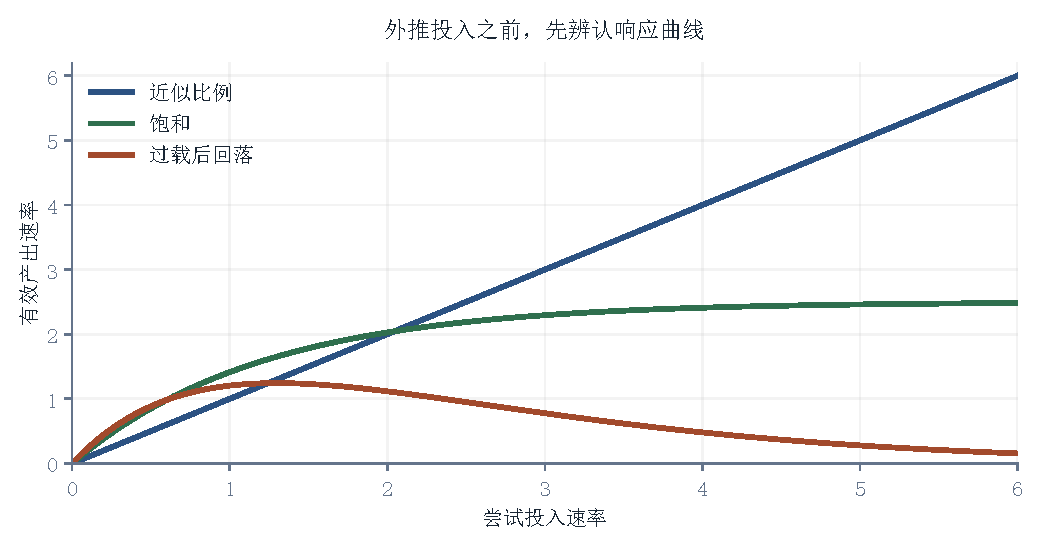
\includegraphics[width=\textwidth]{figures/response-regimes.pdf}
\caption{投入与有效产出可以近似成比例、逐渐饱和，也可以在过载后回落。曲线为机制示意，具体系统的形式与参数需要测量。}
\label{fig:mechanism-response-regimes}
\end{figure}
\subsection{速率失配与界面耗散}

\subhead{三套时钟不能同频}

上一节分开讲的三条响应谱之间，还有一个更隐蔽的问题：它们不能用同一种速度逻辑驱动。比特可以高频生成，原子需要功率匹配，生命需要弛豫时间。智能进入现实系统时，不只是进入不同介质，也是在穿过不同速率的界面。比特层可以在极短时间内计算、更新和传播；原子层有惯性、传热、摩擦、疲劳、执行器响应和安全边界；生命层还有代谢周期、免疫反应、组织修复、行为适应和长期反馈。输入层越快，越不能假定吸收层会同步变快。

这里会出现一种类似阻抗失配的现象。在工程系统中，源端与负载端如果阻抗不匹配，输入能量不能有效传入负载，反而会产生反射、损耗或振荡。这一关系的标准形式是反射系数
\begin{equation}
\Gamma=\frac{Z_L-Z_S}{Z_L+Z_S},\qquad \frac{P_{\mathrm{refl}}}{P_{\mathrm{in}}}=|\Gamma|^2
\end{equation}
这里以无损传输线接终端负载为例，$Z_S$表示实数正的特性阻抗，$Z_L$表示负载阻抗，单位为欧姆。$\Gamma$是电压反射系数，反射功率与入射功率之比为$|\Gamma|^2$；负载也取非负实数时，$\Gamma$位于$-1$与$1$之间。阻抗匹配使反射消失。智能系统中的输出频率、审核吞吐和执行能力各有单位，需另行测量；排队、丢弃、过调节和结构损伤则是失配可以直接观察的结果。

失配可以用输入速率与吸收能力之比描述。设$r=v_{\mathrm{in}}/v_{\mathrm{abs}}$，以吸收能力为单位记录有效推进量，另用损伤项描述超载后的退化：
\begin{equation}
r=\frac{v_{\mathrm{in}}}{v_{\mathrm{abs}}},
\qquad
u(r)=
\begin{cases}
r, & 0<r\le 1\\[3pt]
1-\kappa\,(r-1)^{m}, & r>1
\end{cases}
\label{eq:rate-mismatch}
\end{equation}
$v_{\mathrm{in}}$和$v_{\mathrm{abs}}$采用相同单位，$r$无量纲。$u$是净推进速率除以吸收能力所得的相对量。$r\le1$时输入全部被吸收，$u=r$表示能力尚未用满；$r>1$时，模型以$\kappa(r-1)^m$表示超载引起的净损失。$\kappa\ge0$、$m>0$须由观察确定，$u<0$表示损伤超过当期收益。若系统只排队而不退化，应改用饱和吞吐模型。信息网络、机械装置和生命系统都可能在超载后受损，差别须由具体机制与数据说明。

分层转换在工程系统里早有成熟的做法。电网的频率控制不是单一回路：一次调频由发电机组调速器在秒级自动完成，二次调频由调度中心在分钟级调整出力计划，三次调频和机组组合则在小时到天的尺度上重新排布。层级越慢，能调动的资源越多，代价也越高；把慢层的问题压给快层，系统会失稳，把快层的问题堆到慢层，则会积压。数据系统中的安排同类：写入先落到日志里，再由批处理合并进主存储，读取请求不会被要求等待所有维护动作完成。这些结构承认的都是同一件事，源端和负载端的速率不同，中间必须有人做转换，转换本身要消耗资源，但不做转换的代价更大。

成熟的 AI 系统不是把所有介质推向最高频率，而是建立跨介质的速率转换。真正的智能不是单纯提高源端输出，而是提高源端与负载端之间的匹配效率。AI 不一定失败在模型不够强，也可能失败在界面不匹配：输出太多，系统无法筛选；更新太快，流程无法吸收；控制太密，物理层开始振荡；干预太强，生命系统开始反弹；指标太频繁，组织开始内耗。\key{智能没有消失，而是在界面处被耗散了。}
\begin{figure}[ht]
\centering
% >>>>>>>>>> figs/fig-rate-mismatch.tex >>>>>>>>>>
% 图 3-2  速率失配：两侧都是浪费，只是浪费的形式不同
% 横轴是「输入速率 ÷ 介质吸收速率」的对数刻度，纵轴是有效转化率。
% 三条曲线对应三种介质：比特的吸收带最宽，原子次之，生命最窄。
% 左侧（输入慢于吸收）是产能闲置；右侧（输入快于吸收）是界面耗散——
% 堆积、发热、磨损。生命介质在右侧还跌破零：不是不转化，是被反噬。
% 坐标宏里不写括号（见 fig-three-media.tex 的注释）。
\begin{tikzpicture}[x=1cm, y=1cm, font=\small,
  ax/.style={-{Stealth[length=2.0mm]}, ink, line width=0.6pt},
  tk/.style={font=\scriptsize, text=slate, anchor=north},
  yk/.style={font=\scriptsize, text=slate, anchor=east}
]
\useasboundingbox (-0.35,0.95) rectangle (11.70,-5.60);

\def\aX{1.05} \def\aY{-4.00} \def\dx{1.70} \def\dy{2.85}
\def\px#1{\aX+\dx*2.5+\dx*#1}
\def\py#1{\aY+\dy*#1}

% ---------- 两侧失配区（先铺底）----------
\fill[deepblue!8] (\aX,{\aY-0.10}) rectangle ({\px{0}},{\aY+\dy*1.20});
\fill[rust!9]     ({\px{0}},{\aY-0.10}) rectangle ({\px{2.5}},{\aY+\dy*1.20});
\node[font=\scriptsize\heiti, text=deepblue!80, anchor=north] at ({\px{-1.35}},{\aY+\dy*1.16})
      {闲置：输入慢于吸收};
\node[font=\scriptsize\heiti, text=rust!85, anchor=north] at ({\px{1.30}},{\aY+\dy*1.16})
      {耗散：输入快于吸收};

% ---------- 坐标轴 ----------
\draw[ax] (\aX,\aY) -- ({\px{2.5}+0.30},\aY)
      node[anchor=south east, font=\scriptsize, text=ink, yshift=2pt] {输入速率 / 吸收速率};
\draw[ax] (\aX,\aY) -- (\aX,{\aY+\dy*1.24})
      node[anchor=south, font=\scriptsize, text=ink, yshift=1pt] {相对净推进量};
\foreach \e/\t in {-2.5/{$10^{-2.5}$},0/{$1$},2.5/{$10^{2.5}$}} {
  \node[tk] at ({\px{\e}},{\aY-0.10}) {\t};
}
\foreach \f in {0,0.5,1.0} {
  \draw[slate!55, line width=0.4pt] (\aX,\py{\f}) -- ({\aX-0.07},\py{\f});
  \node[yk] at ({\aX-0.09},\py{\f}) {\f};
}
% 零线（生命介质的代偿会跌破它）
\draw[slate!70, line width=0.6pt] ({\aX-0.05},\aY) -- ({\px{2.5}+0.30},\aY);
% 匹配线
\draw[slate!65, line width=0.6pt, dashed] (\px{0},\aY) -- (\px{0},{\aY+\dy*1.20});
\node[font=\scriptsize, text=slate, anchor=west] at ({\px{0}+0.09},{\aY+0.13}) {匹配};

% ---------- 三条响应曲线 ----------
\def\ptsA{}
\foreach \e/\f in {-2.5/0.10, -2.0/0.24, -1.5/0.43, -1.0/0.65, -0.5/0.83,
                   0.0/0.94, 0.5/0.90, 1.0/0.79, 1.5/0.65, 2.0/0.53, 2.5/0.43} {
  \pgfmathsetmacro{\xx}{\aX+\dx*2.5+\dx*\e}
  \pgfmathsetmacro{\yy}{\aY+\dy*\f}
  \xdef\ptsA{\ptsA\space(\xx,\yy)}
}
\draw[deepblue!85, line width=1.7pt] plot[smooth, tension=0.85] coordinates {\ptsA};

\def\ptsB{}
\foreach \e/\f in {-2.5/0.03, -2.0/0.10, -1.5/0.23, -1.0/0.44, -0.5/0.70,
                   0.0/0.90, 0.5/0.84, 1.0/0.65, 1.5/0.42, 2.0/0.26, 2.5/0.17} {
  \pgfmathsetmacro{\xx}{\aX+\dx*2.5+\dx*\e}
  \pgfmathsetmacro{\yy}{\aY+\dy*\f}
  \xdef\ptsB{\ptsB\space(\xx,\yy)}
}
\draw[terra!90, line width=1.7pt] plot[smooth, tension=0.85] coordinates {\ptsB};

\def\ptsC{}
\foreach \e/\f in {-2.5/0.01, -2.0/0.05, -1.5/0.14, -1.0/0.32, -0.5/0.60,
                   0.0/0.86, 0.4/0.86, 0.8/0.62, 1.2/0.22, 1.5/0.00,
                   2.0/-0.22, 2.5/-0.34} {
  \pgfmathsetmacro{\xx}{\aX+\dx*2.5+\dx*\e}
  \pgfmathsetmacro{\yy}{\aY+\dy*\f}
  \xdef\ptsC{\ptsC\space(\xx,\yy)}
}
\draw[forest!85, line width=1.7pt] plot[smooth, tension=0.85] coordinates {\ptsC};

% ---------- 曲线右端贴签 ----------
\node[font=\scriptsize, text=deepblue!85, anchor=west] at ({\px{2.5}+0.12},{\py{0.43}})
      {比特};
\node[font=\scriptsize, text=terra!90, anchor=west] at ({\px{2.5}+0.12},{\py{0.17}})
      {原子};
\node[font=\scriptsize, text=forest!85, anchor=west] at ({\px{2.5}+0.12},{\py{-0.34}})
      {生命};

% ---------- 读数：同一速率下差距可以很大 ----------
\draw[ink!50, line width=0.45pt, densely dotted] (\px{1.0},\aY) -- (\px{1.0},{\aY+\dy*0.79});
\draw[ink!50, line width=0.45pt, densely dotted] ({\px{1.0}},{\aY+\dy*0.79}) -- ({\px{0.0}},{\aY+\dy*0.79});
\node[font=\scriptsize, text=ink, anchor=north east, align=right]
      at ({\px{0.98}},{\py{0.76}}) {同一输入速率下\\净推进量可能不同};
\draw[ink!55, line width=0.5pt, {Stealth[length=1.4mm]}-{Stealth[length=1.4mm]}]
      ({\px{1.0}},{\aY-0.42}) -- ({\px{0.0}},{\aY-0.42});
\end{tikzpicture}

% <<<<<<<<<< figs/fig-rate-mismatch.tex <<<<<<<<<<

\caption{速率失配：两侧都是浪费，只是形式不同。横轴为输入速率与吸收速率之比，比值偏离中点越远，失配越大。三条曲线分属三种介质，可用带宽依次收窄；纵轴为相对净推进量，负值表示超载损伤超过有效推进；三条线采用不同示意参数。}
\label{fig:rate-mismatch}
\end{figure}


\subhead{介质适配}

因此，AI 时代成熟的智能观，不能只问模型能否输出更优结果，而要问输出如何被介质转译。它是否稳定，还是引发震荡？是否低耗，还是制造废热和维护负担？是否可控，还是触发生命与系统反弹？是否可验证，还是只在表示空间中看似成立？智能的边界不只在模型内部，也在介质响应之中。介质响应谱的意义，正在于纠正一种无介质的智能幻想：AI 不是把答案直接写进世界，而是把输出交给介质，比特会把它扩散，原子会要求它做功，生命会对它反馈，每一种转译都有成本，每一种响应都有边界，每一种吸收都有失败形式。

真正有效的智能系统，必须学会适配介质。面对比特，它要处理真实性和信任；面对原子，它要处理功率、耗散和维护；面对生命，它要处理反馈、弛豫和长期后果。它不能只会生成，还必须知道生成之后将被什么吸收；不能只会优化，还必须知道优化进入介质后会变成什么残余；不能只会加速，还必须知道何时需要降频、缓冲和验证。本章开头那句话到这里才算落到实处：智能不是直接改变世界，而是被介质转译，而 AI 的真实效能，取决于这种转译是否稳定、低耗、可控、可验证。

网络协议提供了同类经验的另一个版本。1980 年代中期的互联网出现过拥塞崩溃，从劳伦斯伯克利实验室到加州大学伯克利分校的一条链路，吞吐量一度从 32 千比特每秒掉到 40 比特每秒。Van Jacobson 和 Michael Karels 在 1988 年给出的解决办法不是在接收端扩容，而是给发送端加一个拥塞窗口：发送端在收到确认之前只能发送有限的数据，丢包被解释为路径拥塞的信号，窗口随之减半，平稳时再缓慢增长\cite{jacobson1988}。这个设计承认的正是源端必须服从吸收端。如果发送端只按自己的输出能力推进，中间节点的队列会先被填满，然后开始丢弃，两端重传进一步加重负担，系统的有效吞吐量反而下降。协议的自律不是道德要求，而是把介质的带宽写进了源端的控制律。

但介质并不是等待被适配的空白材料。每一种介质都有自己的历史，它被制造出来的时候，参照的是人的身体、既有的工艺和当时的制度，而不是智能的输入格式。智能进入这样的介质时，真正的问题往往不是转译发生在哪一层，而是能不能在不改动介质骨架的条件下完成转译；而骨架一旦需要改动，代价就要按原子世界的方式支付。
